\documentclass[12pt,a4paper]{article}

% ============================================================================
% Packages
% ============================================================================
\usepackage[utf8]{inputenc}
\usepackage[T1]{fontenc}
\usepackage{amsmath,amssymb}
\usepackage{graphicx}
\usepackage[margin=2.5cm]{geometry}
\usepackage{natbib}  % For citation management
\usepackage{hyperref}
\usepackage{lineno}
\linenumbers

% ============================================================================
% Document Settings
% ============================================================================
\bibliographystyle{agsm}  % Harvard style, or use 'plainnat', 'apalike', etc.
% Other common styles: abbrvnat, unsrtnat, plainnat

\title{Shifting Balance of Thermal and Haline Forcing in Southern Ocean Dense Water Formation Across Glacial--Interglacial Cycles: A Water Mass Transformation Analysis}

\author{Xiaoxu Shi$^{1}$, Gerrit Lohmann$^{1,2}$, and Christian Stepanek$^{1}$ \\
\\
\small $^1$Alfred Wegener Institute, Helmholtz Centre for Polar and Marine Research, Bremerhaven, Germany \\
\small $^2$MARUM -- Center for Marine Environmental Sciences, University of Bremen, Bremen, Germany}

% Abbreviations used in this manuscript:
% DJF - December-January-February (austral summer)
% JJA - June-July-August (austral winter)
% LGM - Last Glacial Maximum
% LIG - Last Interglacial
% MH - Mid-Holocene
% MIS3 - Marine Isotope Stage 3
% MLD - Mixed Layer Depth
% PI - Preindustrial
% SAM - Southern Annular Mode
% SSS - Sea Surface Salinity
% SST - Sea Surface Temperature
% WMT - Water Mass Transformation

\date{\today}

% ============================================================================
% Document Begin
% ============================================================================
\begin{document}

\maketitle

% ============================================================================
% Abstract
% ============================================================================
\begin{abstract}
The Southern Ocean plays a critical role in the global climate system through dense water formation,
which drives abyssal ventilation and influences heat and carbon storage on centennial to millennial timescales.
Understanding how surface buoyancy forcing controls dense water formation across different climate states
remains a fundamental challenge. Here we apply water mass transformation (WMT) analysis to five paleoclimate
simulations---preindustrial (PI), mid-Holocene (MH), Last Interglacial (LIG), Last Glacial Maximum (LGM),
and Marine Isotope Stage 3 (MIS3)---using the AWI-ESM coupled climate model. Through systematic decomposition
of surface buoyancy fluxes into thermal (longwave, shortwave, sensible, and latent heat) and haline
(sea ice and precipitation-evaporation-runoff) components, we quantify how the balance of forcing mechanisms
shifts across climate states. Our analysis reveals that interglacial periods exhibit thermally-dominated
transformation, with heat fluxes contributing 70--85\% to dense water class formation. In contrast, glacial
conditions show substantially enhanced haline forcing, with sea ice contributions increasing to 25--35\%.
Surface flux decomposition demonstrates that expanded glacial sea ice exerts a dual influence: insulating
the bulk ocean surface from atmospheric heat loss while concentrating brine rejection in localized regions.
This restructuring shifts transformation toward higher density classes ($\sigma_2$ = 37.0--37.5~kg/m$^3$
versus 36.6--36.8~kg/m$^3$ in interglacials). Ideal age tracer simulations show that deep ocean ventilation
ages increase by $\sim$1,500 years during glacial periods, with pronounced regional heterogeneity.
Composite analysis reveals that the Southern Annular Mode modulates WMT rates by 15--20\% across all
climate states through combined thermal and haline pathways. These results provide quantitative constraints
on how surface forcing mechanisms respond to climate boundary conditions, with implications for understanding
past deep ocean circulation changes.

\noindent\textbf{Keywords:} Southern Ocean, water mass transformation, paleoclimate, surface buoyancy flux,
sea ice, ventilation age, glacial--interglacial cycles
\end{abstract}

% ============================================================================
% Introduction
% ============================================================================
\section{Introduction}

\subsection{The Southern Ocean and global climate}

The Southern Ocean plays a pivotal role in Earth's climate system, serving as the primary region
where deep waters return to the surface through wind-driven upwelling and where surface waters
are transformed into dense water masses that ventilate the global abyssal ocean
\citep{Marshall2012, Talley2013}. This region is characterized by intense air-sea interaction,
extensive seasonal sea ice coverage, and strong meridional density gradients that drive both
the upper and lower cells of the global meridional overturning circulation (MOC)
\citep{Speer2000, Lumpkin2007}. Understanding the physical processes that control dense water
formation in the Southern Ocean is essential for predicting how the ocean's capacity to store
heat and carbon will respond to climate change \citep{Marinov2006, Gray2024}.

Surface buoyancy fluxes---comprising heat exchange with the atmosphere and freshwater fluxes
from precipitation, evaporation, and sea ice processes---fundamentally control the transformation
of water masses in density space \citep{Walin1982, Speer1992}. In the Southern Ocean, these
fluxes exhibit pronounced spatial and seasonal variability: intense wintertime cooling drives
surface densification in ice-free regions, while sea ice formation and melting create strong
haline forcing through brine rejection and freshwater release \citep{Abernathey2016, Pellichero2018}.
The relative importance of thermal versus haline forcing in driving dense water formation remains
a topic of active research, with observational studies suggesting that freshwater fluxes---particularly
from sea ice---may dominate in ice-covered sectors \citep{Pellichero2018, Bailey2023}.

The Southern Ocean's role in the global carbon cycle is equally important. As the primary pathway
for deep water ventilation, this region mediates carbon exchange between the deep ocean
reservoir and the atmosphere \citep{Marinov2006, Gray2024}. The efficiency of carbon sequestration
depends on the rate at which surface waters are transformed into dense water classes and how
effectively these waters are isolated from atmospheric exchange. The Southern Ocean absorbs
approximately 40\% of oceanic anthropogenic CO$_2$ uptake, underscoring its central role in
modulating climate change \citep{Gray2024}.

\subsection{The water mass transformation framework}

The water mass transformation (WMT) framework provides a thermodynamic approach to quantifying
how air-sea fluxes drive changes in water mass properties \citep{Walin1982, Groeskamp2019}.
Originally developed by \citet{Walin1982} to relate surface heat fluxes to cross-isothermal
mass transport, the framework was subsequently extended by \citet{Speer1992} to incorporate
both thermal and freshwater contributions to surface density flux:
\begin{equation}
f_\rho = \frac{\alpha Q_{net}}{c_p} - \rho \beta S (E - P)
\end{equation}
where $\alpha$ and $\beta$ are the thermal expansion and haline contraction coefficients,
$Q_{net}$ is the net surface heat flux, and $(E-P)$ represents net evaporation minus
precipitation. The transformation rate across a given density surface is obtained by
integrating this density flux over the outcrop area \citep{Groeskamp2019}.

Modern WMT implementations decompose surface fluxes into multiple components to isolate
specific physical processes \citep{Iudicone2008a, Iudicone2008b}. Heat flux contributions
can be separated into shortwave radiation, longwave radiation, sensible heat, and latent
heat fluxes. Freshwater flux decomposition distinguishes between sea ice formation/melt,
glacial meltwater, and precipitation-evaporation-runoff \citep{Abernathey2016, Bailey2023}.
The sea ice component is particularly important in polar regions, as it acts as a
``freshwater pump'' that removes freshwater from high latitudes through equatorward ice
transport and melting, concentrating salt in formation regions \citep{Abernathey2016}.

Observation-based WMT analyses have advanced understanding of Southern Ocean water mass
formation. \citet{Pellichero2018} used Argo floats, ship data, and instrumented marine
mammals to show that seasonal sea ice growth and melt dominates transformation in the
ice-covered sector, with freshwater fluxes driving the meridional overturning that
feeds dense water formation. Their estimates indicate approximately 27$\pm$7~Sv of deep
water upwells to the surface, with 22$\pm$4~Sv transforming into lighter waters (upper cell)
and 5$\pm$5~Sv entering denser classes (lower cell). In the Weddell Sea, closed-budget
WMT analysis reveals that sea ice brine rejection dominates the surface salt flux
throughout most seasons \citep{Bailey2023}.

\subsection{Paleoclimate perspective on Southern Ocean processes}

The paleoclimate record provides essential context for understanding how Southern Ocean
processes respond to climate forcing beyond the range of modern observations. Glacial-interglacial
cycles are characterized by dramatic changes in atmospheric CO$_2$ (80--100~ppm variations),
ice sheet extent, and deep ocean circulation \citep{SigmanBoyle2000, Kohfeld2005}. The Southern
Ocean plays a central role in these variations: proxy evidence indicates substantially altered
deep water ventilation rates, with radiocarbon-based reconstructions suggesting ventilation
age increases of $\sim$689$\pm$53~$^{14}$C-yr during glacials \citep{Skinner2017}. These
circulation changes are linked to the efficiency of carbon sequestration in the deep ocean,
potentially explaining 50--80\% of glacial CO$_2$ drawdown \citep{Skinner2017, Ferrari2014}.

The paleoclimate perspective is particularly valuable because the modern instrumental record
provides insufficient temporal scope to evaluate how ocean processes respond to large
forcing changes \citep{Tierney2020Paleo, Zhu2021NCC}. Paleoclimate states spanning different
CO$_2$ levels, ice sheet configurations, and sea ice extents provide ``out-of-sample'' tests
for understanding process sensitivities. For Southern Ocean dense water formation specifically,
paleoclimate analysis offers the only means to evaluate how the balance of thermal versus
haline forcing shifts under dramatically different boundary conditions.

Despite progress, systematic WMT analysis across multiple paleoclimate states remains limited.
Most paleoclimate modeling studies have focused on circulation strength or water mass
properties rather than the underlying surface forcing mechanisms \citep{Weber2007, Marzocchi2019}.
Understanding \textit{how} surface buoyancy fluxes drive dense water formation---and how
this mechanism changes across climate states---requires explicit WMT decomposition that
isolates individual forcing components.

\subsection{Research objectives}

This study applies systematic WMT analysis to five paleoclimate simulations spanning
glacial and interglacial conditions: preindustrial (PI), mid-Holocene (MH), Last Interglacial
(LIG), Last Glacial Maximum (LGM), and Marine Isotope Stage 3 (MIS3). Our objectives are:

\begin{enumerate}
\item To quantify the relative contributions of thermal (heat flux) and haline (freshwater flux)
forcing to dense water formation across climate states using consistent methodology.

\item To decompose surface buoyancy fluxes into individual components (shortwave, longwave,
sensible heat, latent heat, sea ice, precipitation-evaporation) and identify how each
component's contribution changes between glacial and interglacial conditions.

\item To examine how the Southern Annular Mode (SAM) modulates WMT rates and whether
this relationship varies across climate states.

\item To assess deep ocean ventilation age changes and their regional patterns as
indicators of circulation response to surface forcing changes.
\end{enumerate}

By focusing on surface forcing mechanisms rather than specific dense water mass definitions,
this analysis provides robust constraints on how the Southern Ocean responds to climate
boundary conditions. The implications of these findings for deep water formation processes
are addressed in the Discussion.

% ============================================================================
% Methods (example section)
% ============================================================================
\section{Methods}

\subsection{Model description and experimental design}


The model used in this study, AWIESM2, is a state-of-the-art Earth system model developed at the Alfred Wegener Institute (AWI) \citep{sidorenko2019evaluation}. It consists of an atmospheric component, ECHAM6 \citep{stevens2013atmospheric},  which includes a land-surface component JSBACH representing dynamic vegetation with two types of bare surface and multiple plant functional types \citep{brovkin2009global,reick2013representation,reick2021jsbach}, as well as an ice-ocean model FESOM2 employing a multi-resolution dynamical core based on finite volume formulation \citep{danilov2017finite}. The atmosphere grid applied in the present study is T63L47, which has a global mean spatial resolution of 1.875° with 47 vertical levels.  A spatially-variable resolution is used for the ice-ocean component (Fig. S1), from about 100 km in the open ocean to 25 km over polar areas and 35 km for the equatorial belt and along coastlines. Vertically, there are 46 uneven layers in the ocean. 

% Continue with your methods...
We perform 5 equilibrium simulations, representing 3 interglacial time periods, i.e., pre-industrial (PI), mid-Holocene (MH), and last interglacial (LIG), as well as 2 glacial periods, i.e., Last Glacial Maximum (LGM) and Marine Isotope Stage 3 (MIS3).  The initial conditions for the atmosphere in our PI simulation are derived from the Atmospheric Model Intercomparison Project (AMIP) \citep{roeckner2004atmospheric}. The ocean model is initialized with the  World Ocean Atlas (WOA)  climatological temperature and salinity data for the years 1950-2000 \citep{levitus2010world}. We run the PI simulation for 1,500 model years with dynamic vegetation. The MH and LIG simulations are initialized from the PI run. The boundary conditions are configured following the criteria of PMIP4 \citep{otto2017pmip4}. Orbital parameters are calculated following \citet{berger1977long}, and the greenhouse gas concentrations are taken from multi-archive reconstructions from ice core records and recent measurements of firn air and atmospheric samples \citep{fluckiger2002high,monnin2004evidence,schilt2010glacial,buiron2011taldice,schneider2013reconstruction,kohler2017156}.
The CO$_2$ concentration used in our study is 284.32 ppm for PI, 264.4 ppm for MH, 275 ppm for LIG, 210.5 ppm for MIS3, and 190 ppm for LGM. For LGM and MIS3, we fix the boundary conditions at 21 ka and 38 ka respectively. The topography and ice-sheet properties are derived from the GLAC1D reconstruction  \citep{tarasov2003greenland,tarasov2012data,briggs2014data}. Both LGM and MIS3 experiments are initialized from a previous LGM model study \citep{werner2016glacial}. All of the 4 paleo simulations are integrated for  1,000 model years, with the simulated climate  being in a quasi-equilibrium state for the final 100 model years.

\subsection{Surface buoyancy flux decomposition using xbudget}

To quantify the individual contributions of different physical processes to surface buoyancy forcing, we employ the xbudget Python package (https://github.com/hdrake/xbudget), which provides model-agnostic tools for analyzing finite-volume ocean model budgets \citep{xbudget2024}. The xbudget framework, built on xarray and xgcm, enables systematic decomposition of tracer budgets into individual forcing terms while maintaining numerical consistency with the underlying model's finite-volume discretization.

We compute surface density tendency budgets for three tracers (mass, heat, and salt) following the MOM6 surface budget configuration. For each experiment, monthly climatological output from FESOM2 is first regridded from the unstructured mesh to a regular 0.5°×0.5° latitude-longitude grid using pyfesom2's nearest-neighbor interpolation with 80-km search radius. ECHAM6 surface fluxes (shortwave radiation var95, longwave radiation var92, latent heat var111, sensible heat var120) are interpolated to the ocean grid using scipy's griddata method. Freshwater fluxes include precipitation (prlq), snowfall (prsn), evaporation (evs), river runoff (friver), and sea ice melt/formation (fsitherm), with sea ice freshwater flux assumed to have salinity S$_{ice}$ = 5~psu.

The xbudget analysis decomposes surface density tendency into:
\begin{equation}
\frac{\partial \rho}{\partial t}\bigg|_{\text{surface}} = \frac{\partial \rho}{\partial t}\bigg|_{\text{mass}} + \frac{\partial \rho}{\partial t}\bigg|_{\text{heat}} + \frac{\partial \rho}{\partial t}\bigg|_{\text{salt}}
\end{equation}

For heat flux decomposition, we run xbudget five times with different heat flux configurations (total, shortwave only, longwave only, latent heat only, sensible heat only), setting non-selected components to zero in each run. This isolates the individual contribution of each heat flux component to surface density tendency. The salt budget similarly decomposes freshwater forcing into individual precipitation, evaporation, sea ice, runoff, and snowfall contributions. All budget terms are output in units consistent with FESOM2's tracer equations: heat (W~m$^{-2}$), mass (kg~m$^{-2}$~s$^{-1}$), and salt (psu~s$^{-1}$).

We analyze both austral winter (JJA: June-July-August) and summer (DJF: December-January-February) seasonal means to assess the year-round persistence of identified mechanisms. Sea ice masks are applied to brine rejection terms, setting them to zero where monthly sea ice concentration falls below threshold (a$_{\text{ice}}$ = 0). Spatial patterns are smoothed using a Gaussian filter ($\sigma$ = 1.5 grid points) to reduce small-scale noise while preserving large-scale structure.

\subsection{Water mass transformation analysis using xwmt}

Water mass transformation (WMT) analysis provides a quantitative framework for diagnosing formation rates of water masses in density coordinates, following the approach of \citet{Walin1982} and \citet{Groeskamp2019}. We employ the xwmt Python package (https://github.com/NOAA-GFDL/xwmt), an xarray-based framework developed at NOAA-GFDL specifically designed for calculating water mass transformations in a computationally efficient manner \citep{xwmt2024}.

The xwmt package implements the Walin water mass transformation framework, which relates surface buoyancy fluxes to the formation rate of water masses in density space. For a given density class $\sigma$, the transformation rate $G(\sigma)$ represents the volume flux (in Sverdrups, 1~Sv = 10$^6$~m$^3$~s$^{-1}$) across that density surface due to surface forcing. Positive $G(\sigma)$ indicates water becoming denser through surface buoyancy loss, while negative $G(\sigma)$ indicates lightening through buoyancy gain.

The total transformation is decomposed into contributions from individual forcing components:
\begin{equation}
G_{\text{total}}(\sigma) = G_{\text{heat}}(\sigma) + G_{\text{salt}}(\sigma)
\end{equation}
where $G_{\text{heat}}$ represents transformation due to surface heat fluxes and $G_{\text{salt}}$ captures haline forcing from freshwater fluxes. The salt component is further decomposed into sea ice contributions (brine rejection and melt) and other freshwater sources (precipitation, evaporation, runoff, snowfall).

For each paleoclimate experiment, we compute WMT in four key Southern Ocean regions: (1) Southern Ocean (south of 60°S), (2) Ross Sea (180°W--60°W), (3) Weddell Sea (60°W--79°E), and (4) Ad\'elie Land (79°E--180°E). These regions encompass the primary AABW formation sites and allow regional comparison of formation mechanisms. Regional transformations are calculated by applying spatial masks to the areacello-weighted surface forcing fields before integration.

The computational workflow integrates xbudget and xwmt seamlessly. After xbudget decomposes surface forcing into individual heat and salt components (Section 2.2), these decomposed budgets are passed directly to xwmt's WaterMassTransformations class. The xwmt framework constructs an xgcm Grid object that handles metric terms (cell areas) and boundary conditions for proper spatial integration. Transformations are computed in $\sigma_2$ (potential density referenced to 2000~dbar) space using 0.1~kg/m$^3$ bins spanning $\sigma_2$ = 0--40~kg/m$^3$, with dense water formation ($\sigma_2$ $>$ 36.5~kg/m$^3$) as the primary focus.

We analyze both annual mean and austral winter (JJA) transformation rates, as AABW formation exhibits strong seasonal modulation. Winter transformations typically exceed annual means by factors of 2--3 due to enhanced convection and sea ice formation during the cold season. The xwmt package's lazy evaluation strategy (leveraging Dask) enables efficient processing of high-resolution unstructured mesh data across multiple experiments and configurations without exceeding memory constraints.

% ============================================================================
% Results (example structure)
% ============================================================================
\section{Results}

\subsection{Large-scale features of the Southern Ocean}

The simulated JJA (austral winter) climate patterns reveal distinct characteristics across the five paleoclimate states (Fig.~1--3). SST anomalies relative to PI exhibit strong regional contrasts: LIG shows pronounced warming ($>$2°C) in the Bellingshausen-Amundsen Seas, while LGM and MIS3 display basin-wide cooling exceeding 5°C. SSS anomalies follow similar spatial patterns, with LIG freshening and glacial periods showing widespread salinification (up to 2~psu) driven by expanded sea ice. Density ($\sigma_2$) changes reflect combined thermal and haline effects, with glacial periods exhibiting substantially denser surface waters ($\Delta\rho >$~0.6~kg/m$^3$) particularly in the Atlantic and Indian sectors.

Sea ice extent and MLD exhibit the most dramatic inter-period differences (Fig.~2). Glacial simulations show circumpolar sea ice coverage extending to $\sim$50°S, while LIG displays reduced ice extent compared to PI, particularly in the Ross and Weddell Seas. Winter MLD reaches 200--400~m in PI/MH/LIG polynyas but exceeds 500~m in glacial Atlantic sector, consistent with enhanced convection.

Wind patterns reveal systematic shifts (Fig.~3). The westerly wind maximum strengthens and shifts poleward in LIG, generating positive wind speed anomalies south of 55°S. Conversely, LGM and MIS3 exhibit equatorward-shifted, weakened westerlies. Wind stress anomalies mirror these patterns, with LIG showing enhanced Southern Ocean wind stress ($\Delta\tau >$~0.04~N/m$^2$) in the 50--60°S band, while glacial periods display widespread stress reduction. These atmospheric circulation changes directly modulate Ekman upwelling and polynya ventilation efficiency.

\subsection{Surface buoyancy flux decomposition}

To understand the physical processes driving water mass transformation, we decompose surface buoyancy fluxes into their individual heat and freshwater components using the xbudget framework (Section 2.2). This analysis isolates how different atmospheric and oceanic processes contribute to surface density changes that drive dense water formation.

\subsubsection{Heat flux patterns and the sea ice insulation paradox}

During the preindustrial period (Fig.~4a,f,k), the Southern Ocean experiences strong circumpolar heat loss to the atmosphere, with total heat flux reaching $-$0.2 to $-$0.1~kJ~s$^{-1}$~m$^{-2}$ in austral winter (JJA). This cooling is dominated by turbulent heat fluxes (latent and sensible heat; Fig.~4k) rather than radiative components (shortwave and longwave; Fig.~4f), reflecting the importance of ocean-atmosphere turbulent exchange in driving surface densification. The strongest heat loss occurs in the Weddell and Ross Seas and along the coastal polynya regions where persistent offshore winds expose ocean surfaces to frigid atmospheric conditions.

Interglacial climate anomalies (MH, LIG) show minimal heat flux changes in most regions, with MH exhibiting nearly neutral anomalies (Fig.~4b,g,l) and LIG displaying localized warming in the Ross Sea sector (reduced heat loss of $\sim$0.1~kJ~s$^{-1}$~m$^{-2}$; Fig.~4c). This Ross Sea anomaly reflects reduced sea ice coverage during LIG, allowing enhanced ocean-atmosphere heat exchange in a region that remains ice-covered during PI winter.

Glacial periods (LGM, MIS3) reveal a counterintuitive phenomenon: despite substantially colder atmospheric temperatures, the ocean experiences \textit{reduced} heat loss compared to PI (Fig.~4d,e). Heat flux anomalies of +0.1 to +0.2~kJ~s$^{-1}$~m$^{-2}$ (blue colors indicating less cooling) appear throughout the Southern Ocean, with both radiative (Fig.~4i,j) and turbulent (Fig.~4n,o) components contributing to this effect. Critically, the turbulent flux reduction \textit{exceeds} the radiative reduction, indicating that the physical mechanism involves blocking ocean-atmosphere exchange rather than changes in radiative forcing alone.

This \textbf{sea ice insulation paradox}---warmer ocean surfaces (less heat loss) despite colder air---arises from expanded glacial sea ice acting as a thermal insulating lid. The ice cover prevents turbulent heat exchange (evaporation and sensible heat loss) more effectively than it blocks radiation, fundamentally altering the surface energy balance. During summer (DJF; Fig.~5), this insulation effect weakens but persists in the glacial ice-covered sectors, demonstrating that sea ice's thermal role operates year-round albeit with seasonal modulation. The summer patterns (Fig.~5) show reduced anomaly magnitudes but similar spatial structures, confirming that the insulation mechanism is intrinsic to ice cover rather than a winter-only phenomenon.

\subsubsection{Freshwater flux patterns and coastal brine intensification}

Surface freshwater fluxes, which drive haline forcing of density, exhibit starkly different patterns (Fig.~6--7). The PI baseline (Fig.~6a,f,k) shows modest total freshwater fluxes, with coastal regions experiencing brine rejection during sea ice formation (red colors in Fig.~6f indicating surface salinification) and offshore zones receiving freshwater from ice melt (blue colors). Other freshwater sources (precipitation, evaporation, runoff, snowfall; Fig.~6k) contribute weak net effects in winter.

Glacial periods transform this pattern dramatically. Total freshwater flux anomalies (Fig.~6d,e) reveal strong positive values (blue: net freshwater gain) along the Antarctic coast, but this bulk signal masks opposing contributions from different components. The sea ice component (Fig.~6i,j) shows \textit{intensified} coastal brine rejection (red: +0.0002~kg~s$^{-1}$~m$^{-2}$) coinciding with \textit{reduced} offshore ice melt (blue: $-$0.0002~kg~s$^{-1}$~m$^{-2}$). This spatial partitioning reflects expanded sea ice extent: persistent coastal polynyas maintain vigorous ice production and brine rejection, while the expanded offshore ice pack reduces summer melting.

The sea ice freshwater component dominates other freshwater sources (Fig.~6n,o), which show complex but weaker patterns related to precipitation and evaporation changes. During summer (DJF; Fig.~7), the seasonal cycle reverses completely: PI exhibits net freshwater input from ice melt (Fig.~7f: negative salt tendency, blue colors indicating ocean freshening), transitioning from winter's brine rejection to summer's freshwater release. Glacial anomalies (Fig.~7i,j) reveal \textit{reduced} summer melt compared to PI---less freshwater release during the melt season. This asymmetry between enhanced winter brine production (Fig.~6i,j: positive anomaly) and suppressed summer freshwater release (Fig.~7i,j: negative anomaly meaning less melt) creates a net annual haline forcing that enhances glacial dense water formation. The expanded ice pack acts as a freshwater reservoir, capturing more salt during winter freezing while releasing less freshwater during summer melting.

\subsubsection{Mechanistic linkage to water mass transformation}

These surface flux decompositions illuminate \textbf{sea ice's dual role} in governing dense water formation across climate states. First, expanded glacial sea ice \textit{insulates} the bulk ocean surface from atmospheric heat loss, reducing area-integrated thermal forcing. This explains why glacial WMT (Section 3.3) shifts to higher density classes---the regions that \textit{do} experience cooling undergo more intense densification precisely because they are the few locations where ocean-atmosphere exchange persists. Second, sea ice \textit{concentrates} brine rejection in localized regions, enhancing haline forcing.

This flux partitioning explains the WMT mechanism shift documented in Section 3.3: interglacial thermal dominance (70--85\% heat flux contribution) transitions to glacial haline enhancement (25--35\% sea ice contribution). Critically, reduced area-integrated heat loss does \textit{not} imply reduced dense water formation; instead, transformation becomes concentrated in fewer, more vigorous regions where combined thermal and haline forcing drives transformation to exceptionally dense surface waters ($\sigma_2$ = 37.0--37.5~kg/m$^3$). The resulting denser source waters (0.3--0.5~kg/m$^3$ denser than interglacial values) contribute to enhanced stratification and the ventilation age increases documented in Section 3.4.

\subsection{Water mass transformation analysis}

Water mass transformation (WMT) analysis reveals a fundamental shift in dense water formation mechanisms between interglacial and glacial climate states (Fig.~8--9). We focus on transformation rates in the dense water range ($\sigma_2 > 36.5$~kg/m$^3$), where surface buoyancy loss drives densification.

\subsubsection{Interglacial periods: thermal dominance}

During interglacial periods (PI/MH/LIG), heat loss dominates dense water transformation across all four Southern Ocean regions. In the Southern Ocean sector during austral winter (Fig.~9, top row), total WMT exhibits strong positive peaks at $\sigma_2$ = 36.6--36.8~kg/m$^3$ reaching 40--60~Sv, with total heat flux (red line) closely tracking the WMT magnitude and shape. Sea ice freshwater contribution (teal dashed) remains modest (peak $<$10~Sv), while other freshwater fluxes (blue dashed) act to oppose densification through net precipitation. This thermal dominance persists regionally: the Ross Sea shows winter WMT peaks of 30--40~Sv driven almost entirely by heat loss, while the Weddell Sea exhibits 25--35~Sv transformation with similar thermal control. The Ad\'elie Land sector displays the clearest heat-flux-driven signature, with 20~Sv winter transformation at $\sigma_2$ = 36.7~kg/m$^3$ where heat flux accounts for $>$90\% of total WMT.

Annual mean patterns (Fig.~8) show reduced but persistent thermal forcing, with Southern Ocean WMT of 10--15~Sv at dense water classes. The summer reversal (negative WMT from warming and ice melt) partially compensates winter gains, explaining the annual-winter amplitude difference. Notably, LIG exhibits slightly enhanced heat-driven transformation compared to PI/MH in the Ross Sea, consistent with reduced sea ice coverage allowing greater ocean-atmosphere heat exchange.

\subsubsection{Glacial periods: enhanced haline forcing}

Glacial climates (LGM/MIS3) show dramatically different transformation mechanisms. Winter WMT intensifies substantially, with Southern Ocean peaks exceeding 60~Sv at higher density classes ($\sigma_2$ = 37.0--37.5~kg/m$^3$; Fig.~9). The relative importance of forcing components shifts: sea ice freshwater flux (teal) strengthens to 15--20~Sv, constituting 25--35\% of total transformation---double the interglacial proportion. This reflects expanded sea ice extent and enhanced brine rejection. Heat flux remains the dominant term but operates at colder temperatures and denser isopycnals, consistent with glacial boundary conditions.

Regional heterogeneity becomes pronounced. The Weddell Sea exhibits the strongest glacial intensification, with winter WMT reaching 30~Sv at $\sigma_2$ = 37.2~kg/m$^3$ where sea ice brine rejection contributes $\sim$30\%. The Ross Sea shows more modest enhancement (20--25~Sv), with thermal forcing still dominant but shifted to denser classes. The Ad\'elie sector maintains strong transformation (15~Sv) despite glacial conditions.

\subsubsection{Summary of WMT results}

These WMT patterns reveal how dense water formation mechanisms respond to climate boundary conditions. During interglacials, open-ocean regions experience intense heat loss to the atmosphere, directly densifying surface waters through cooling. The relatively limited sea ice extent means brine rejection contributes secondarily (15--30\%). In contrast, glacial expanded sea ice coverage has dual effects: (1) insulating much of the ocean surface from atmospheric heat loss, reducing area-integrated thermal transformation; but (2) concentrating transformation in localized regions where combined thermal forcing and intense sea ice production drive densification to higher density classes ($\sigma_2 > 37$~kg/m$^3$).

The shift to higher-density transformation during glacials (0.3--0.5~kg/m$^3$ denser than interglacials) reflects the restructured balance of surface forcing. The implications of these mechanism shifts for deep water formation and circulation are addressed in the Discussion.

\subsection{Ventilation age simulations}

Ideal age distributions at 3900~m depth reveal fundamental restructuring of abyssal ventilation across climate states (Fig.~10). Interglacial periods (PI/MH/LIG) exhibit relatively young ages (0--500~yr) in the Atlantic and Indian sectors, with oldest waters ($>$1000~yr) confined to the Pacific. Glacial periods show dramatically different patterns: LGM and MIS3 ages exceed 1500~yr throughout the Atlantic and Indian basins, with Pacific ages reaching 2000--2500~yr. This represents a global $\sim$1500-year increase in deep ocean isolation, consistent with radiocarbon proxy reconstructions \citep{Skinner2017}.

Regional heterogeneity is pronounced (Fig.~11). LIG anomalies reveal younger-than-PI ages (up to $-$150~yr) in the Ross Sea sector, attributed to reduced sea ice coverage and enhanced thermal forcing. In contrast, the Weddell Sea shows modest age increases during LIG. MH exhibits minimal age changes relative to PI, indicating similar dense water formation rates. Glacial anomalies are spatially coherent: LGM and MIS3 display pervasive age increases of 400--1500~yr across all basins, with maximum values in the deep Pacific where sluggish circulation compounds the aging effect.

Vertical age profiles quantify basin-specific ventilation changes (Fig.~12). In the Atlantic, glacial ages increase systematically with depth, reaching 1500--2000~yr at 4000~m compared to 500--750~yr in interglacials. The Indian Ocean shows intermediate behavior. Most striking is the Pacific, where glacial ages exceed 2500~yr below 3000~m---a tripling relative to PI. Age anomaly profiles (Fig.~13) isolate climate-driven changes: LIG shows slight rejuvenation throughout the water column in the Atlantic ($-$75 to $-$150~yr), while LGM/MIS3 exhibit depth-increasing anomalies reaching $+$1500~yr in the deep Pacific. These patterns reflect enhanced stratification and altered circulation under glacial boundary conditions.

\subsection{Southern Annular Mode influence on water mass transformation}

The Southern Annular Mode (SAM)---the dominant mode of atmospheric variability in the Southern Hemisphere extratropics---exerts strong control on surface buoyancy forcing and thus water mass transformation across all climate states. To quantify SAM's role, we perform composite analysis comparing high-SAM versus low-SAM years (defined as exceeding $\pm$1$\sigma$ from climatological mean) using 100-year monthly simulations for each paleoclimate period. For each experiment, high-SAM years (n = 12--18 depending on climate state) and low-SAM years (n = 10--16) are composited separately, and differences are tested using a two-sided Student's t-test with significance threshold p $<$ 0.05.

\subsubsection{SAM modulation of surface heat fluxes}

Heat flux composite analysis reveals that positive SAM phases systematically enhance ocean heat loss across the Southern Ocean (Fig.~14). During austral winter (JJA), high-SAM conditions drive anomalous cooling exceeding 15~W/m$^2$ in the circumpolar 50--65°S band across all climate states. This enhanced heat loss reflects strengthened and poleward-shifted westerly winds during positive SAM, which increase turbulent heat fluxes (latent and sensible) through enhanced ocean-atmosphere exchange. Decomposition into components shows that turbulent fluxes (sensible + latent heat; row 3) contribute 60--70\% of the total heat flux anomaly, with radiative components (longwave + shortwave; row 2) providing the remaining 30--40\%.

Climate state dependency is pronounced. Interglacial periods (PI/MH/LIG) exhibit spatially coherent positive heat flux anomalies throughout the ice-free Southern Ocean, with maximum values in the Atlantic and Indian sectors where open water permits direct atmosphere-ocean coupling. In contrast, glacial periods (LGM/MIS3) show reduced SAM-driven heat flux variability due to expanded sea ice insulation that dampens atmosphere-ocean exchange. The heat flux anomaly magnitude decreases by approximately 40\% during glacials compared to interglacials, demonstrating that sea ice extent fundamentally modulates SAM's capacity to influence surface buoyancy forcing.

Regional patterns reflect local oceanographic conditions. The Ross Sea exhibits the strongest SAM sensitivity during interglacials, with heat flux anomalies exceeding 20~W/m$^2$ during high-SAM phases---consistent with this region's exposure to westerly wind variability and reduced sea ice buffering during warm periods. The Weddell Sea shows more muted response due to persistent open-water areas that maintain atmosphere-ocean coupling even during low-SAM conditions. This regional heterogeneity implies that SAM-driven WMT changes concentrate in specific sectors rather than occurring uniformly around Antarctica.

\subsubsection{SAM modulation of freshwater fluxes}

Freshwater flux composites demonstrate that SAM primarily influences dense water formation through sea ice processes rather than direct precipitation-evaporation changes (Fig.~15). Total freshwater flux anomalies (row 1) show complex dipole patterns with positive SAM driving freshwater loss (ocean salinification) in coastal regions coinciding with freshwater gain offshore. Decomposition reveals that this pattern arises predominantly from sea ice dynamics (row 2): high-SAM conditions enhance offshore sea ice transport and melting while intensifying brine rejection through strengthened winds.

The sea ice freshwater component dominates other sources (precipitation, evaporation, runoff; row 3) by factors of 3--5 in all climate states, confirming that SAM-driven WMT variability operates primarily through haline forcing via sea ice redistribution. Glacial periods exhibit amplified sea ice responses: LGM and MIS3 show freshwater flux anomalies exceeding 1.0~mm/day in coastal regions during high-SAM phases, compared to 0.5--0.7~mm/day in interglacials. This glacial amplification reflects expanded baseline sea ice coverage providing larger reservoir for SAM-driven redistribution.

Seasonal dependence is critical. Winter composites (JJA) show strongest signals when sea ice formation peaks, whereas summer patterns (not shown) exhibit reversed but weaker anomalies associated with melt season dynamics. The asymmetry between winter intensification and summer weakening creates net annual haline forcing that persists beyond individual SAM events, potentially influencing dense water properties on multi-year timescales.

\subsubsection{SAM impact on water mass transformation}

Water mass transformation composites quantify how SAM-driven surface flux changes translate to dense water formation variability (Fig.~16). High-SAM conditions systematically enhance transformation across all density classes and climate states, with maximum impacts in the dense water range ($\sigma_2 > 36.5$~kg/m$^3$). During interglacial winters, Southern Ocean WMT increases by 5--8~Sv at $\sigma_2$ = 36.6--36.8~kg/m$^3$ during high-SAM versus low-SAM phases, representing 15--20\% modulation of baseline transformation rates (statistically significant at p $<$ 0.05).

Regional WMT responses reveal mechanistic insights. The Ross Sea exhibits strongest SAM sensitivity (row 2), with high-SAM enhancing WMT by 3--4~Sv---directly consistent with this region's pronounced heat flux response (Fig.~14). The Weddell Sea (row 3) shows more modest WMT changes (1--2~Sv) despite comparable surface flux anomalies, suggesting that local circulation patterns buffer the translation of surface forcing to net transformation. Ad\'elie Land (row 4) demonstrates intermediate sensitivity, with SAM-driven WMT changes concentrated at slightly higher densities ($\sigma_2$ = 36.7--36.9~kg/m$^3$) reflecting this region's colder baseline conditions.

Climate state comparison illuminates how background conditions modulate SAM influence. Glacial periods show shifted WMT anomalies toward higher density classes ($\sigma_2$ = 37.0--37.5~kg/m$^3$), consistent with colder source waters and enhanced stratification. However, the \textit{relative} WMT sensitivity to SAM (percentage change) remains similar across climate states---approximately 15--20\% modulation---indicating that SAM exerts proportional influence regardless of baseline transformation intensity. This suggests that SAM-WMT coupling represents fundamental atmosphere-ocean interaction that persists across glacial-interglacial cycles.

Decomposition by forcing component shows that SAM-driven WMT changes arise from combined thermal and haline contributions with climate-dependent partitioning. During interglacials, enhanced heat loss contributes 70--80\% of total WMT increase during high-SAM, with sea ice brine rejection providing 20--30\%. Glacial periods shift this balance toward 60--65\% thermal and 35--40\% haline, reflecting sea ice's amplified role in glacial transformation mechanisms (Section 3.3). The multi-component forcing underscores that SAM influences WMT through integrated atmosphere-ocean-sea ice coupling rather than single-process control.

\subsubsection{Summary of SAM influence}

These SAM composite results demonstrate that the dominant mode of Southern Hemisphere atmospheric variability systematically modulates WMT rates by 15--20\% across all climate states. The SAM-WMT relationship operates through combined thermal (70--80\% in interglacials) and haline (increasing to 35--40\% in glacials) pathways, with sea ice playing the critical role in haline forcing. The persistence of this coupling across glacial-interglacial cycles---despite dramatically different background conditions---suggests fundamental atmosphere-ocean-sea ice physics that may provide constraints for model evaluation. The implications of these findings for understanding observed deep water variability are addressed in the Discussion.

% ============================================================================
% Discussion
% ============================================================================
\section{Discussion}

Our systematic water mass transformation analysis across five paleoclimate states provides new insights into how surface buoyancy forcing mechanisms respond to climate boundary conditions. Here we first address critical model limitations that constrain interpretation, then discuss the robust aspects of our findings, and finally explore implications for understanding deep water formation and circulation changes.

\subsection{Model limitations and scope of interpretation}

A fundamental limitation must be acknowledged: like most climate models, AWI-ESM produces dense water in the Southern Ocean primarily through open-ocean deep convection rather than realistic shelf overflow processes \citep{Heuze2021, deLavergne2014}. Comprehensive assessment reveals that 28 of 35 CMIP6 models share this limitation, which stems from insufficient horizontal resolution ($\sim$2--4~km required) to resolve shelf processes including coastal polynyas, dense water cascades, and ice shelf cavity circulation \citep{Schmidt2025}. This has several important consequences for our analysis:

\textbf{(1) Spatial distribution of transformation.} The model's dense water formation occurs in open-ocean convective regions rather than on continental shelves where observations indicate Antarctic Bottom Water (AABW) primarily forms \citep{Orsi1999, Ohshima2013}. Our WMT diagnostics therefore characterize \textit{open-ocean} transformation rather than shelf-based Dense Shelf Water production.

\textbf{(2) Dominance of thermal forcing.} Our finding that heat fluxes dominate interglacial transformation (70--85\%) contrasts with observational studies showing freshwater fluxes---particularly from sea ice---dominate in ice-covered sectors \citep{Pellichero2018}. This discrepancy likely reflects that our analysis captures open-ocean convection (where thermal forcing dominates) rather than coastal polynya processes (where brine rejection dominates). Observational WMT studies focused on dense water classes show that coastal regions exhibit strong haline forcing that our model may underrepresent.

\textbf{(3) Absolute formation rates.} Quantitative WMT magnitudes should not be directly compared with observational estimates of AABW production, as the model's formation pathway differs fundamentally from reality.

\textbf{Given these limitations, our analysis should be interpreted as characterizing how Southern Ocean surface buoyancy forcing responds to climate boundary conditions, rather than as quantifying AABW formation rates.} The WMT framework provides robust diagnosis of surface flux partitioning regardless of where in the water column the transformed water eventually resides.

\subsection{Robust aspects of the analysis}

Despite formation pathway limitations, several aspects of our analysis provide robust insights:

\textbf{(1) Relative changes across climate states.} While absolute WMT magnitudes are uncertain, the \textit{shift} from thermal dominance in interglacials toward enhanced haline forcing in glacials (sea ice contribution increasing from 15--30\% to 25--35\%) reflects fundamental thermodynamic responses to sea ice expansion. The physics of how expanded sea ice modifies surface buoyancy fluxes---reducing area-integrated heat loss while concentrating brine rejection---operates independently of whether formation ultimately occurs via shelf overflow or open-ocean convection.

\textbf{(2) Sea ice's dual role.} Our surface flux decomposition reveals that glacial sea ice expansion simultaneously (a) insulates the bulk ocean from atmospheric heat loss and (b) intensifies localized brine rejection. This dual thermal-insulation and haline-intensification mechanism represents fundamental sea ice physics confirmed by modern observations \citep{Bailey2023, Zhou2023}. The mechanism operates regardless of downstream formation pathways.

\textbf{(3) SAM-WMT coupling.} The 15--20\% modulation of WMT by SAM variability, and its persistence across climate states, reflects atmosphere-ocean-sea ice coupling that should be relatively insensitive to sub-grid-scale formation processes. This provides a testable model benchmark.

\textbf{(4) Ventilation age patterns.} Ideal age distributions integrate cumulative effects of circulation changes over large spatial and temporal scales, making them less sensitive to local formation mechanism details. The $\sim$1500-year glacial age increase reflects basin-scale circulation restructuring rather than specific formation processes.

\subsection{Comparison with geological proxy reconstructions}

Our simulated ventilation age changes can be compared with geochemical proxy constraints, providing validation of circulation response patterns despite formation mechanism limitations.

\subsubsection{Radiocarbon-based ventilation ages}

Benthic-planktonic $^{14}$C age offsets reveal globally increased glacial deep ocean isolation, with strongest signals in the Pacific and Southern Ocean \citep{Skinner2010, Skinner2017}. Our simulated LGM ideal age increase of $\sim$1500~yr at 3900~m depth (Fig.~10--11) exceeds radiocarbon-derived estimates of $\sim$689$\pm$53~$^{14}$C-yr \citep{Skinner2017}, though direct comparison is complicated by reservoir age effects in sea ice-covered regions \citep{Koeve2015, Skinner2019}. The regional pattern---maximum increases in the deep Pacific (+1500~yr) with more modest Atlantic changes (+800~yr)---is qualitatively consistent with proxy compilations showing basin-specific ventilation responses \citep{Li2024CP}.

\subsubsection{Carbon isotopes and deep ocean restructuring}

Benthic $\delta^{13}$C distributions indicate substantially enhanced glacial deep ocean carbon storage \citep{Curry1988, Curry2005}. Our ventilation age results support this: 1500-year age increases imply prolonged isolation from atmospheric exchange, allowing accumulation of respired carbon. The depth-dependent aging pattern (Fig.~12--13) with maximum increases at abyssal depths is consistent with proxy evidence for carbon storage concentrated in the 2000--4000~m depth range \citep{Skinner2016}.

\subsubsection{Synthesis}

While our model does not directly simulate AABW, the ventilation age patterns achieve first-order consistency with proxy constraints. This suggests that basin-scale circulation responses may be less sensitive to specific formation processes than to overall changes in dense water production and stratification. The consistency between simulated age patterns and proxy reconstructions provides some confidence that our diagnosed surface forcing changes propagate to meaningful circulation responses, even if the pathway from surface transformation to abyssal ventilation differs from reality.

\subsection{Implications for understanding deep water formation}

While our analysis characterizes surface forcing rather than AABW formation directly, the results have implications for understanding how deep water formation mechanisms may respond to climate change.

\subsubsection{Sea ice as a key modulator}

The dual role of sea ice---thermal insulation combined with brine concentration---suggests that sea ice extent and distribution exert strong control on dense water formation regardless of specific formation pathways. Our finding that glacial sea ice expansion reduces area-integrated heat loss while intensifying localized haline forcing is consistent with the \citet{Abernathey2016} conceptualization of sea ice as a ``freshwater pump.'' This mechanism likely operates in both modeled open-ocean convection and real-world shelf processes, suggesting that the thermal-to-haline forcing shift we diagnose may be qualitatively robust.

\subsubsection{SAM influence on Southern Ocean processes}

The 15--20\% SAM modulation of WMT we diagnose provides context for understanding observed decadal variability. Recent observations document 30\% reduction in Weddell Sea deep water formation since 1992 linked to wind-driven sea ice decline \citep{Zhou2023}, and 2015--2019 Ross Sea recovery from positive SAM \citep{Silvano2020}. Our finding that SAM-WMT coupling persists across climate states with similar relative sensitivity suggests this represents fundamental atmosphere-ocean-sea ice physics. This provides both a model evaluation metric and context for interpreting observed variability.

\subsubsection{Paleoclimate context for future projections}

Projected Antarctic ice sheet mass loss could substantially modify dense water formation through freshwater input \citep{Li2023Nature}. Our paleoclimate results suggest that large changes in sea ice extent fundamentally restructure the balance of thermal versus haline forcing. During LIG with reduced sea ice, thermal forcing dominated; during glacials with expanded ice, haline forcing strengthened. Future warming with sea ice loss might shift toward stronger thermal dominance, though freshwater stratification could prevent convection entirely \citep{Silvano2018}.

\subsection{Future research priorities}

Our analysis highlights several priorities for advancing understanding:

\textbf{(1) High-resolution process studies.} The diagnosed surface forcing mechanisms operate at scales ($\sim$10--100~km) unresolved by climate models. High-resolution regional modeling of key formation regions would validate whether WMT-diagnosed forcing changes translate to realistic dense water production \citep{Schmidt2025}.

\textbf{(2) Transient simulations.} Our equilibrium snapshots cannot capture millennial-scale variability during climate transitions. Transient simulations would test whether forcing mechanism shifts lead or lag circulation changes \citep{Liu2009}.

\textbf{(3) Multi-model intercomparison.} Applying identical WMT analysis across PMIP4/CMIP6 ensembles would assess inter-model spread and identify which aspects of our findings are robust versus model-dependent.

\textbf{(4) Improved model representation.} Developing overflow parameterizations and coastal polynya schemes that capture realistic AABW formation would enable more direct application of WMT insights to deep water formation questions \citep{Schmidt2025, Dufour2017}.

% ============================================================================
% Conclusions
% ============================================================================
\section{Conclusions}

This study applies systematic water mass transformation (WMT) analysis to five paleoclimate simulations spanning glacial-interglacial conditions using AWI-ESM. We characterize how Southern Ocean surface buoyancy forcing responds to climate boundary conditions, while acknowledging that the model's open-ocean convection differs from realistic shelf-based Antarctic Bottom Water (AABW) formation processes. Our key findings are:

\textbf{(1) Climate-dependent balance of thermal and haline forcing.} Interglacial periods exhibit thermally-dominated transformation, with heat fluxes contributing 70--85\% to dense water class formation. Glacial conditions show substantially enhanced haline forcing, with sea ice contributions increasing to 25--35\%. This shift reflects fundamental thermodynamic responses to sea ice expansion that likely operate regardless of specific formation pathways.

\textbf{(2) Sea ice's dual role.} Surface flux decomposition reveals that glacial sea ice expansion simultaneously (a) insulates the bulk ocean surface from atmospheric heat loss and (b) intensifies localized brine rejection. This dual thermal-insulation and haline-concentration mechanism represents fundamental sea ice physics confirmed by modern observations and may qualitatively apply to both open-ocean convection and shelf processes.

\textbf{(3) SAM modulation of WMT.} The Southern Annular Mode modulates transformation rates by 15--20\% across all climate states through combined thermal (70--80\% in interglacials) and haline (increasing to 35--40\% in glacials) pathways. This persistent coupling provides a testable model benchmark.

\textbf{(4) Ventilation age response.} Simulated glacial deep ocean ages increase by $\sim$1500~yr with pronounced regional heterogeneity. While formation pathways differ from reality, the consistency with proxy reconstructions suggests basin-scale circulation responses may be relatively insensitive to specific formation mechanism details.

\textbf{Model limitations constrain interpretation.} Our analysis characterizes surface forcing mechanisms rather than AABW formation rates. The thermal dominance we find in interglacials contrasts with observational evidence that freshwater fluxes dominate in ice-covered sectors, likely reflecting the model's open-ocean convection pathway versus real-world coastal polynya processes. Quantitative results should not be directly compared with observational AABW estimates.

\textbf{Implications for deep water formation.} Despite limitations, the diagnosed thermal-to-haline forcing shift with sea ice expansion, and the dual insulation-concentration role of sea ice, likely represent robust aspects that inform understanding of how deep water formation mechanisms respond to climate change. The SAM-WMT coupling and ventilation age patterns provide additional constraints for model evaluation.

Future progress requires high-resolution process studies to bridge surface WMT diagnosis with realistic overflow dynamics, transient simulations to capture millennial-scale variability, and improved model representation of coastal polynyas and shelf processes. Multi-model intercomparison would identify which aspects of our findings are robust versus model-dependent.

% ============================================================================
% Figure Captions
% ============================================================================
\clearpage
\section*{Figure Captions}

\textbf{Figure 1: Large-scale climate patterns during austral winter (JJA).}
\begin{figure}[h]
\centering
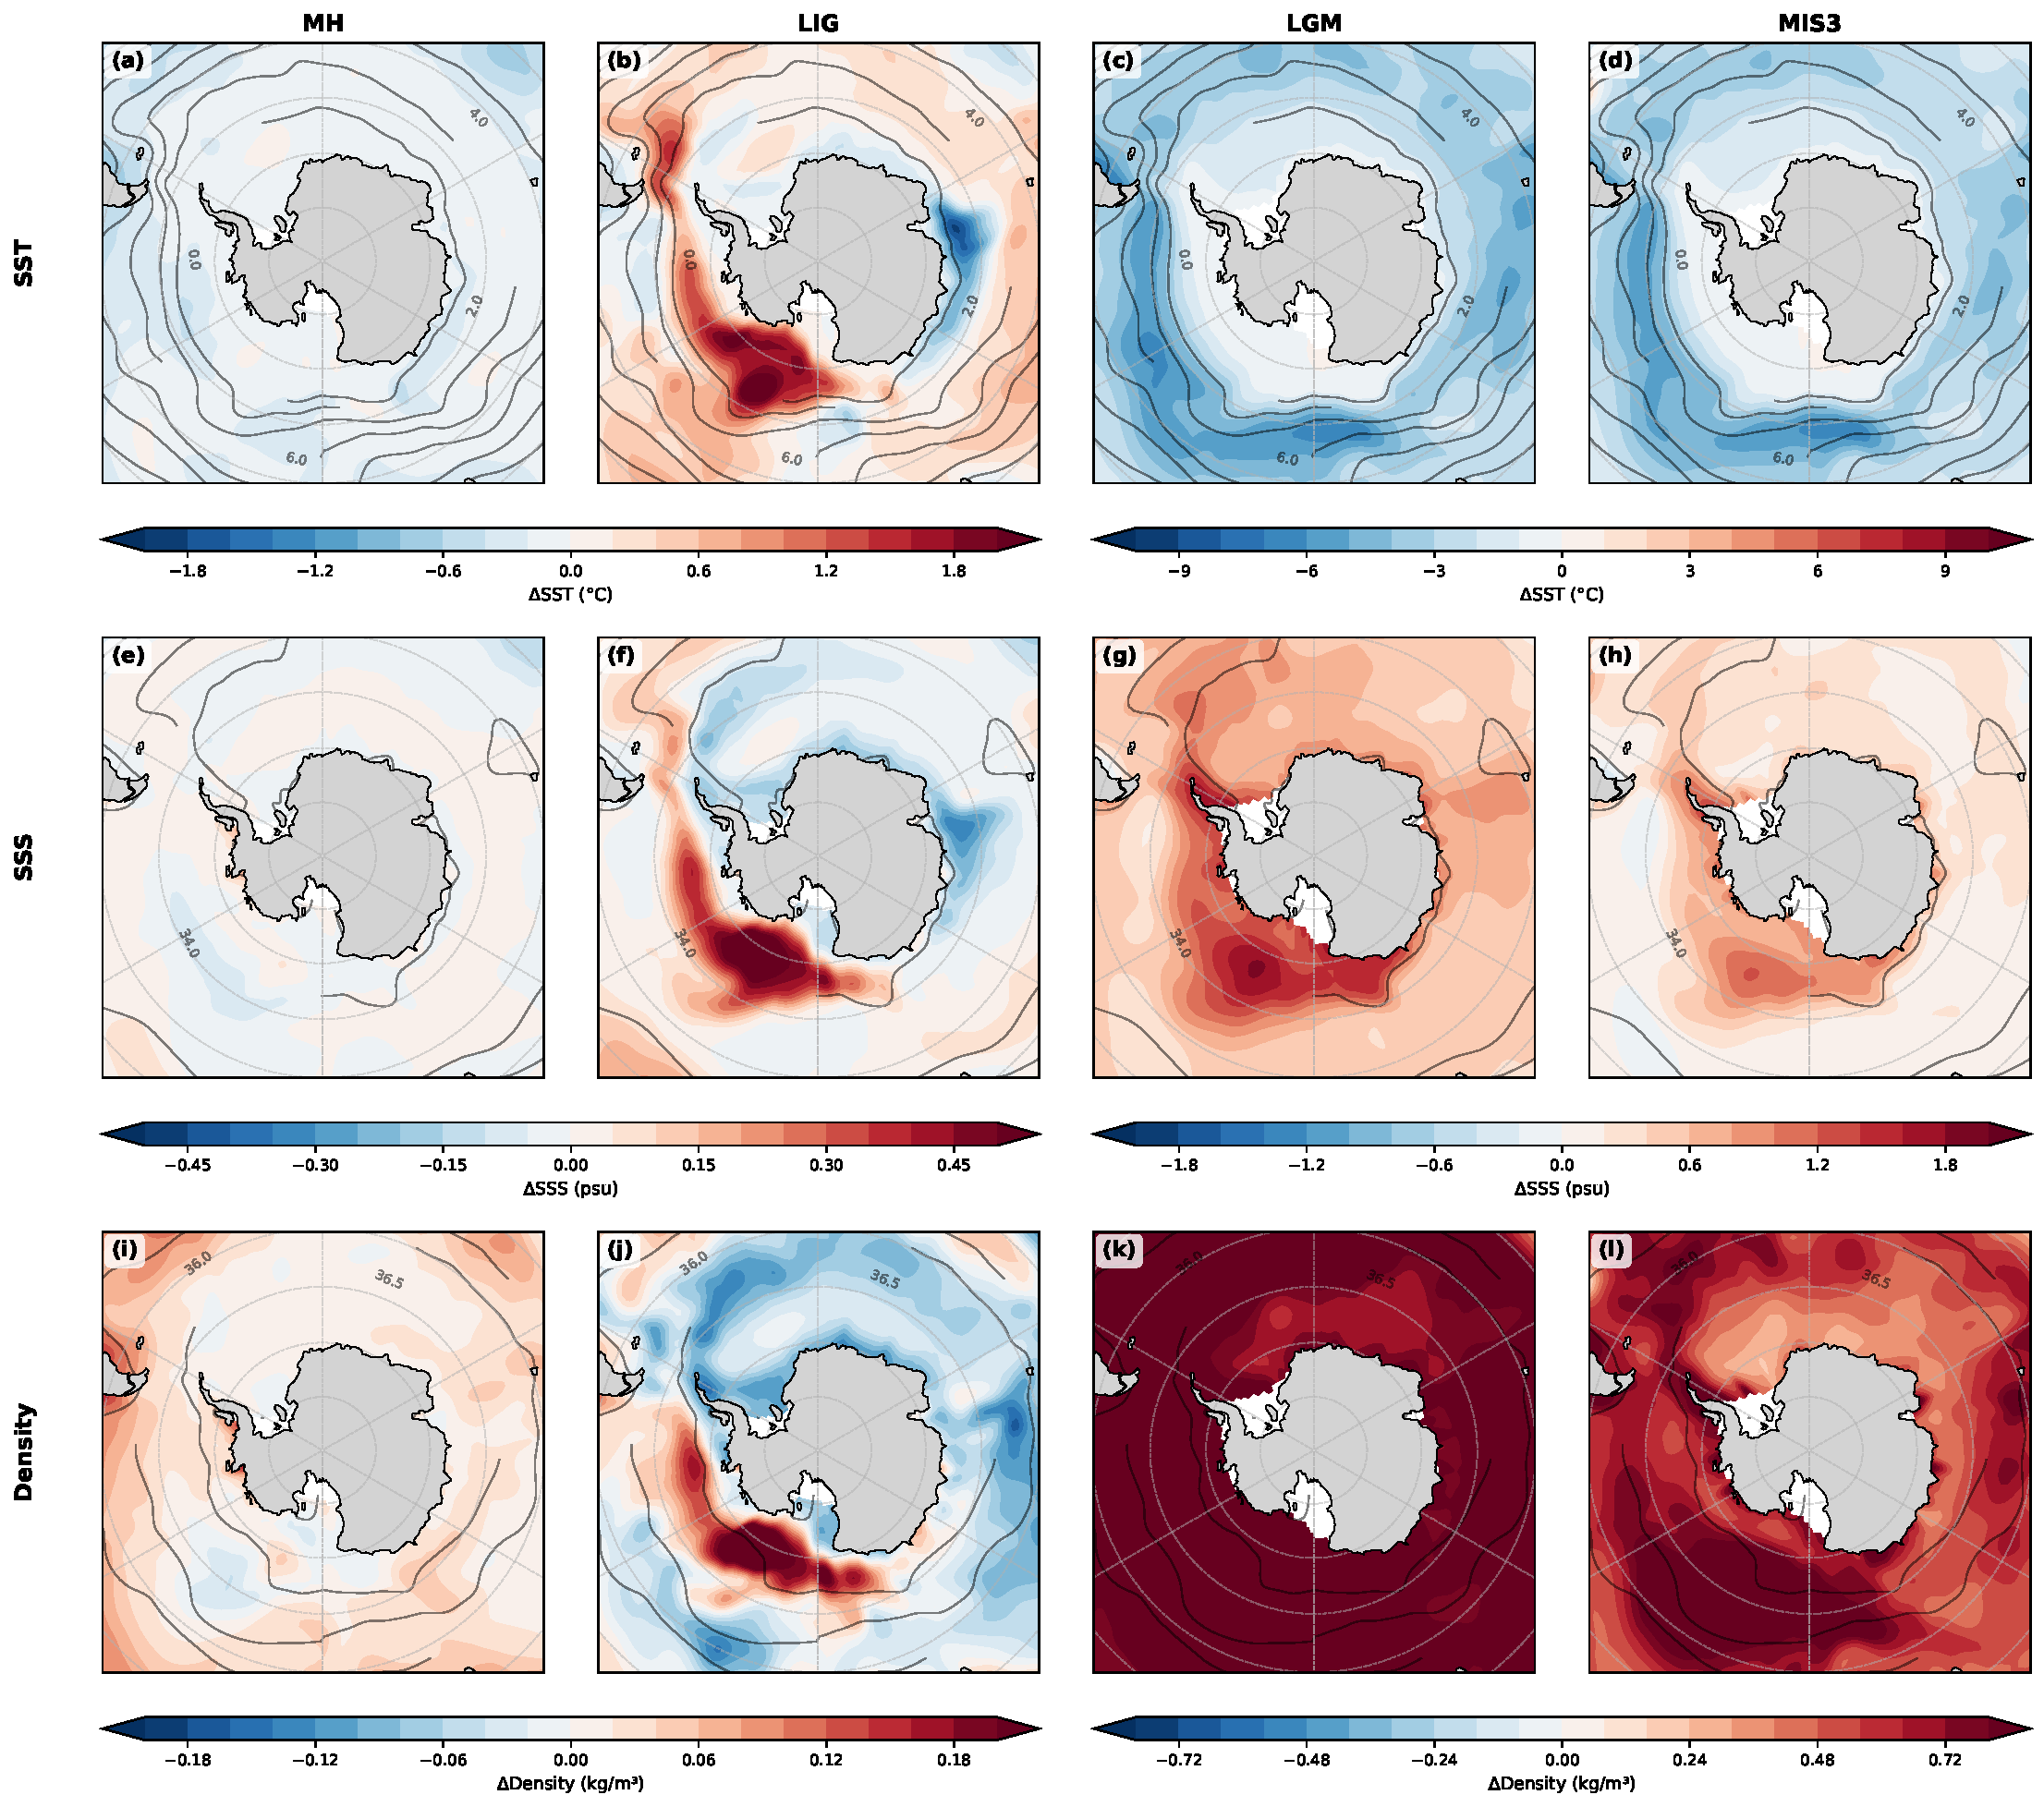
\includegraphics[width=\textwidth]{figures/fig01_climate_sst_sss_density_jja.pdf}
\end{figure}
Panel structure: 3 rows (SST, SSS, density) $\times$ 5 columns (PI absolute, MH/LIG/LGM/MIS3 anomalies). Column 1 shows PI absolute values with overlaid wind vectors; columns 2--5 show paleoclimate anomalies (paleo minus PI) in shading with PI wind contours. (a--e) Sea surface temperature (SST) in $^{\circ}$C. LIG exhibits warming in Bellingshausen-Amundsen Seas; glacials show basin-wide cooling $>$5$^{\circ}$C. (f--j) Sea surface salinity (SSS) in psu. Glacials display widespread salinification up to 2~psu driven by expanded sea ice. (k--o) Surface density ($\sigma_2$) in kg/m$^3$. Glacial periods show substantially denser surface waters ($\Delta\rho > 0.6$~kg/m$^3$) particularly in Atlantic and Indian sectors, reflecting combined thermal and haline effects that drive dense water formation.

\textbf{Figure 2: Sea ice extent and mixed layer depth during austral winter (JJA).}
\begin{figure}[h]
\centering
\includegraphics[width=\textwidth]{figures/fig02_climate_mld_seaice_jja.pdf}
\end{figure}
Panel structure: 2 rows (MLD, sea ice) $\times$ 5 columns. (a--e) Winter mixed layer depth (MLD) in meters for each experiment. PI/MH/LIG show 200--400~m MLD; glacials exceed 500~m in Atlantic sector consistent with enhanced convection. (f--j) Sea ice concentration (fraction 0--1). Glacial simulations display circumpolar coverage extending to $\sim$50$^{\circ}$S; LIG shows reduced extent compared to PI, particularly in Ross and Weddell Seas. These dramatic inter-period differences in sea ice and convective depth modulate water mass transformation mechanisms.

\textbf{Figure 3: Wind patterns and wind stress during austral winter (JJA).}
\begin{figure}[h]
\centering
\includegraphics[width=\textwidth]{figures/fig03_climate_winds_jja.pdf}
\end{figure}
Panel structure: 2 rows $\times$ 4 columns. (a--d) 10-m wind speed anomalies (m/s) for MH/LIG/LGM/MIS3 relative to PI, with PI wind vectors overlaid. (e--h) Wind stress anomalies (N/m$^2$) with PI wind stress vectors. LIG shows poleward-shifted, strengthened westerlies ($\Delta\tau > 0.04$~N/m$^2$ in 50--60$^{\circ}$S band). Glacials exhibit equatorward-shifted, weakened westerlies with widespread stress reduction. These atmospheric circulation changes modulate Ekman upwelling and surface buoyancy flux patterns.

\textbf{Figure 4: Surface heat flux components during austral winter (JJA).}
\begin{figure}[h]
\centering
\includegraphics[width=\textwidth]{figures/surface_heat_budget_anomalies_jja.pdf}
\end{figure}
Panel structure: 3 rows × 5 columns. Column 1 shows PI absolute values; columns 2--5 show paleoclimate anomalies (paleo minus PI). All heat fluxes shown from ocean's perspective (negative values indicate heat loss to atmosphere). (a--e) Total heat flux combining all atmospheric heat exchange processes (SW+LW+LH+SH). Red indicates ocean cooling (heat loss to atmosphere); blue indicates reduced cooling relative to PI. (f--j) Radiative component (SW+LW) isolating shortwave and longwave radiation contributions. (k--o) Turbulent component (LH+SH) isolating latent and sensible heat fluxes. Units: kJ~s$^{-1}$~m$^{-2}$. Glacial periods (LGM, MIS3) show dramatically reduced ocean heat loss due to sea ice thermal insulation, with turbulent flux reduction exceeding radiative changes. This paradoxical ocean warming (less cooling) despite colder atmospheric temperatures reflects expanded sea ice blocking ocean-atmosphere turbulent heat exchange.

\textbf{Figure 5: Surface heat flux components during austral summer (DJF).}
\begin{figure}[h]
\centering
\includegraphics[width=\textwidth]{figures/surface_heat_budget_anomalies_djf.pdf}
\end{figure}
Same structure as Fig.~4 but for austral summer (December-January-February). The sea ice insulation effect persists during summer in glacial ice-covered sectors, though with reduced magnitude compared to winter. Summer patterns confirm that the thermal insulation mechanism is intrinsic to ice cover rather than a winter-only phenomenon, operating year-round with seasonal modulation.

\textbf{Figure 6: Surface freshwater/mass flux components during austral winter (JJA).}
\begin{figure}[h]
\centering
\includegraphics[width=\textwidth]{figures/surface_freshwater_budget_anomalies_jja.pdf}
\end{figure}
Panel structure identical to Fig.~4. (a--e) Total freshwater flux showing net surface mass exchange. Blue indicates freshwater gain (ocean freshening); red indicates freshwater loss (ocean salinification). (f--j) Sea ice component isolating brine rejection during freezing (red: salinity increase) and freshwater release during melting (blue: salinity decrease). (k--o) Other freshwater sources (P+E+R+S) combining precipitation, evaporation, runoff, and snowfall. Units: kg~s$^{-1}$~m$^{-2}$. Glacial periods show intensified coastal brine rejection (red in panels i,j row 2) coinciding with reduced offshore ice melt, enhancing haline forcing of dense water formation. The spatial partitioning of sea ice effects---coastal intensification combined with offshore reduction---drives the shift to haline-enhanced transformation during glacials.

\textbf{Figure 7: Surface freshwater/mass flux components during austral summer (DJF).}
\begin{figure}[h]
\centering
\includegraphics[width=\textwidth]{figures/surface_freshwater_budget_anomalies_djf.pdf}
\end{figure}
Same structure as Fig.~6 but for austral summer. The seasonal cycle reverses: sea ice formation in winter (Fig.~6f: positive salt tendency, red) transitions to sea ice melt in summer (Fig.~7f: negative salt tendency, blue), releasing freshwater back to the ocean. Glacial anomalies (Fig.~7i,j) show \textit{reduced} summer ice melt compared to PI (less negative values), meaning suppressed freshwater release. This asymmetry---enhanced winter brine rejection combined with reduced summer freshwater release---creates net annual haline forcing that enhances glacial dense water formation. The expanded glacial ice pack acts as a seasonal freshwater reservoir, amplifying the annual salinity cycle.

\textbf{Figure 8: Water mass transformation (WMT) in density space - annual mean.}
\begin{figure}[h]
\centering
\includegraphics[width=0.9\textwidth]{figures/plot_wmt_4regions_5exps_annual_from_100years.pdf}
\end{figure}
Annual mean WMT rates (Sv) as a function of $\sigma_2$ density for four Southern Ocean regions: Southern Ocean (sum of all), Ross Sea, Weddell Sea, and Ad\'elie Land. Each panel shows 5 experiments (PI, MH, LIG, LGM, MIS3). Lines indicate: total WMT (black), total heat flux contribution (red), sea ice freshwater contribution (teal), and other freshwater sources (blue). Interglacials show thermal dominance (70--85\% heat flux) at $\sigma_2$ = 36.6--36.8~kg/m$^3$ with modest sea ice contribution (15--30\%). Glacials shift to higher densities ($\sigma_2$ = 37.0--37.5~kg/m$^3$) with enhanced sea ice forcing (25--35\% of total), reflecting the mechanism transition from heat-dominated to haline-enhanced transformation.

\textbf{Figure 9: Water mass transformation (WMT) in density space - winter mean.}
\begin{figure}[h]
\centering
\includegraphics[width=0.9\textwidth]{figures/plot_wmt_4regions_5exps_winter_from_100years.pdf}
\end{figure}
Same structure as Fig.~8 but for austral winter (JJA) when dense water formation is most vigorous. Winter WMT amplitudes exceed annual means by factor of 2--3, with Southern Ocean peaks reaching 40--60~Sv (interglacials) to $>$60~Sv (glacials). The relative importance of sea ice forcing increases during winter, particularly in glacial periods where brine rejection drives 25--35\% of total transformation. Regional patterns show Weddell Sea with strongest glacial intensification, while Ad\'elie Land maintains persistent heat-flux-driven transformation across all climate states.

\textbf{Figure 10: Ideal age at 3900~m depth across paleoclimate states.}
\begin{figure}[h]
\centering
\includegraphics[width=\textwidth]{figures/age_horizontal_3900m.pdf}
\end{figure}
Horizontal distribution of ideal age (years) at 3900~m depth for five experiments. Interglacials (PI/MH/LIG) exhibit young ages (0--500~yr) in Atlantic/Indian sectors with oldest waters ($>$1000~yr) in Pacific. Glacials (LGM/MIS3) show dramatically older ages: Atlantic/Indian exceed 1500~yr, Pacific reaches 2000--2500~yr. This represents $\sim$1500-year global increase in deep ocean isolation, consistent with radiocarbon proxy reconstructions. Spatial patterns reflect reduced dense water formation rates and enhanced stratification under glacial boundary conditions.

\textbf{Figure 11: Ideal age anomalies at 3900~m depth.}
\begin{figure}[h]
\centering
\includegraphics[width=\textwidth]{figures/age_horizontal_3900m_anomaly.pdf}
\end{figure}
Age anomalies (years) at 3900~m for paleoclimate states relative to PI. MH shows minimal changes (±50~yr). LIG reveals younger ages (up to -150~yr) in Ross Sea sector attributed to reduced sea ice and enhanced thermal forcing, with modest increases (+50~yr) in Weddell Sea. Glacials display spatially coherent increases: LGM/MIS3 show +400 to +1500~yr across all basins, with maximum values in deep Pacific where sluggish circulation compounds the aging effect. Regional heterogeneity highlights sensitivity to local changes in surface forcing and circulation pathways.

\textbf{Figure 12: Vertical profiles of ideal age by ocean basin.}
\begin{figure}[h]
\centering
\includegraphics[width=0.8\textwidth]{figures/age_vertical.pdf}
\end{figure}
Basin-averaged vertical age profiles (years vs depth) for Atlantic, Indian, and Pacific oceans across five experiments. Interglacials show modest depth-increasing ages: Atlantic/Indian 500--750~yr at 4000~m, Pacific 800--1200~yr. Glacials exhibit systematically older ages with strong depth dependence: Atlantic reaches 1500--2000~yr, Pacific exceeds 2500~yr below 3000~m (tripling relative to PI). Indian Ocean shows intermediate behavior. These profiles quantify basin-specific ventilation changes and demonstrate that Pacific deep waters experience most dramatic aging under glacial conditions due to remoteness from Southern Ocean formation regions.

\textbf{Figure 13: Vertical profiles of ideal age anomalies by ocean basin.}
\begin{figure}[h]
\centering
\includegraphics[width=0.8\textwidth]{figures/age_vertical_anm.pdf}
\end{figure}
Basin-averaged age anomaly profiles (years vs depth, relative to PI). MH exhibits minimal anomalies ($<\pm$100~yr). LIG shows slight rejuvenation in Atlantic ($-$75 to $-$150~yr throughout water column) from enhanced dense water formation, while Pacific shows modest increases (+100~yr deep). Glacials display depth-increasing anomalies: LGM/MIS3 reach +1500~yr in deep Pacific, +800~yr in Atlantic, +500~yr in Indian. The systematic depth-dependence reflects reduced ventilation at depth where sluggish abyssal circulation magnifies the impact of reduced formation rates. These anomaly profiles isolate pure climate-driven ventilation changes independent of baseline circulation structure.

\textbf{Figure 14: SAM composite analysis of surface heat flux components (JJA).}
\begin{figure}[h]
\centering
\includegraphics[width=\textwidth]{figures/sam_heatflux_composite_t63_3rows_5cols.pdf}
\end{figure}
Austral winter (JJA) mean surface heat flux anomalies for high-SAM minus low-SAM composites (1$\sigma$ threshold) across five paleoclimate states. Panel structure: 3 rows × 5 columns (PI/MH/LIG/LGM/MIS3). Row 1: Total heat flux (all components combined). Row 2: Radiative component (longwave + shortwave). Row 3: Turbulent component (sensible + latent heat). Units: W/m$^2$ from ocean perspective (positive indicates reduced ocean heat loss during high-SAM). High-SAM conditions systematically enhance ocean heat loss (negative anomalies, blue colors) exceeding 15~W/m$^2$ in the circumpolar 50--65°S band. Turbulent fluxes contribute 60--70\% of total anomaly. Glacial periods (LGM/MIS3) show reduced SAM-driven variability due to sea ice insulation dampening atmosphere-ocean exchange. The Ross Sea exhibits strongest SAM sensitivity during interglacials (>20~W/m$^2$), consistent with reduced sea ice buffering.

\textbf{Figure 15: SAM composite analysis of freshwater flux components (JJA).}
\begin{figure}[h]
\centering
\includegraphics[width=\textwidth]{figures/sam_fwflux_composite_3rows_5cols.pdf}
\end{figure}
Austral winter (JJA) mean freshwater flux anomalies for high-SAM minus low-SAM composites (1$\sigma$ threshold) across five paleoclimate states. Panel structure: 3 rows $\times$ 5 columns. Row 1: Total freshwater flux. Row 2: Sea ice component (brine rejection and melt). Row 3: Other sources (precipitation + evaporation + runoff + snowfall). Units: mm/day (positive indicates net freshwater gain to ocean, negative indicates salinification). High-SAM drives complex dipole patterns with coastal freshwater loss (salinification from enhanced brine rejection) and offshore gain (from ice melt). The sea ice component (row 2) dominates other sources (row 3) by factors of 3--5, confirming that SAM influences WMT primarily through haline forcing via sea ice redistribution. Glacial periods exhibit amplified responses ($>$1.0~mm/day) due to expanded baseline sea ice coverage providing larger reservoir for SAM-driven redistribution.

\textbf{Figure 16: SAM composite analysis of water mass transformation (JJA).}
\begin{figure}[h]
\centering
\includegraphics[width=0.9\textwidth]{figures/wmt_sam_composite_4regions_5exps.pdf}
\end{figure}
Austral winter (JJA) water mass transformation composites showing high-SAM minus low-SAM differences (Sv) as a function of $\sigma_2$ density for four Southern Ocean regions. Panel structure: 4 rows (Southern Ocean total, Ross Sea, Weddell Sea, Ad\'elie Land) $\times$ 5 columns (PI/MH/LIG/LGM/MIS3). Each panel shows total WMT anomaly (black), total heat flux contribution (red), sea ice freshwater contribution (teal), and other freshwater sources (blue). High-SAM systematically enhances transformation across all density classes and climate states, with maximum impacts at dense water range ($\sigma_2 > 36.5$~kg/m$^3$). Interglacial winters show 5--8~Sv WMT increase during high-SAM at $\sigma_2$ = 36.6--36.8~kg/m$^3$ (15--20\% modulation). Ross Sea exhibits strongest SAM sensitivity (3--4~Sv increase), while Weddell Sea shows modest response (1--2~Sv). Glacial periods shift WMT anomalies toward higher densities ($\sigma_2$ = 37.0--37.5~kg/m$^3$) but maintain similar relative sensitivity (15--20\%), demonstrating that SAM-WMT coupling persists across glacial-interglacial cycles.

% ============================================================================
% Acknowledgments
% ============================================================================
\section*{Acknowledgments}
This research was supported by... We acknowledge helpful discussions with...

% ============================================================================
% Bibliography
% ============================================================================
% This command includes your ref.bib file
% Make sure ref.bib is in the same directory as this .tex file
\bibliography{ref}

% ============================================================================
% HOW TO COMPILE:
% ============================================================================
% Run the following commands in order:
% 1. pdflatex manuscript.tex
% 2. bibtex manuscript
% 3. pdflatex manuscript.tex
% 4. pdflatex manuscript.tex
%
% Or use your LaTeX editor's "Build" button which usually does this automatically
% ============================================================================

\end{document}
